\documentclass[Ligatures=TeX,table,brazil,svgnames,usetotalslideindicator,compress,10pt]{beamer}

\usetheme[titleformat=allsmallcaps]{metropolis}

\usepackage{polyglossia}
\setdefaultlanguage{brazil}
\disablehyphenation

\usepackage{minted}

\usetikzlibrary{arrows,positioning,calc}

\usepackage{graphicx}
\graphicspath{{./figuras/}}
\usepackage{subcaption}
\usepackage{xmpmulti}

% \usepackage{textpos}

% \usepackage{mdwlist}
% \usepackage{siunitx}
\usepackage{alltt}
% \usepackage{multicol}
\usepackage{xspace}
\usepackage{multirow}
\usepackage{amsmath}

\usepackage{cancel}

\newcommand{\setcoverbg}{
  \setbeamertemplate{background}
  {
\includegraphics[width=\paperwidth,height=\paperheight]{backgrounds/coverbg}}
}
\newcommand{\setintersectionbg}{
  \setbeamertemplate{background}
  {
\includegraphics[width=\paperwidth,height=\paperheight]{backgrounds/blank}}
}
\newcommand{\setsectionbg}{
  \setbeamertemplate{background}
  {
\includegraphics[width=\paperwidth,height=\paperheight]{backgrounds/slidebg2}}
}

\setbeamertemplate{caption}{default}

\title{MCTA025-13 - Sistemas Distribuídos}
\subtitle{Relógios Vetoriais, Exclusão Mútua e Eleição}

\author{Emilio Francesquini}
\institute{Centro de Matemática, Computação e Cognição\\ Universidade Federal do ABC}
\date{06 de agosto de 2018}

\begin{document}

\setcoverbg
\maketitle

\setsectionbg

\begin{frame}
  \frametitle{Disclaimer}
  \begin{itemize}
  \item Estes slides foram preparados para o curso de \textbf{Sistemas
      Distribuídos na UFABC}.
  \item Este material pode ser usado livremente desde que sejam
    mantidos, além deste aviso, os créditos aos autores e
    instituições.
  \item Estes slides foram adaptados daqueles originalmente preparados
    (e gentilmente cedidos) pelo professor \textbf{Daniel Cordeiro, da
      EACH-USP} que por sua vez foram baseados naqueles
    disponibilizados online pelos autores do livro ``Distributed
    Systems'', 3ª Edição em:
    \url{https://www.distributed-systems.net}.
  \end{itemize}
\end{frame}


\begin{frame}
  \frametitle{Relógios Lógicos: a relação ``aconteceu-antes''}

  \begin{block}{A relação ``aconteceu-antes'' (\textit{happened-before})}
    \begin{itemize}
    \item se $a$ e $b$ são dois eventos de um mesmo processo e $a$ ocorreu antes de $b$, então $a \rightarrow b$
    \item se $a$ for o evento de envio de uma mensagem e $b$ for o evento de recebimento desta mesma mensagem, então $a \rightarrow b$
    \item se $a \rightarrow b$ e $b \rightarrow c$, então $a \rightarrow c$
    \end{itemize}
  \end{block}

  \begin{alertblock}{Nota:}
    Isso introduz uma noção de \alert{ordem parcial dos eventos} em um sistema com processos executando concorrentemente.
  \end{alertblock}

\end{frame}

\begin{frame}
  \frametitle{Relógio lógico de Lamport}
  \begin{alertblock}{Problema}
    Como fazemos para manter uma visão global do comportamento do sistema que seja consistente com a relação aconteceu-antes?
  \end{alertblock}

  \begin{block}{Solução}
    Associar um \textit{timestamp} $C(e)$ a cada evento $e$ tal que:
    \begin{description}
    \item[P1] se $a$ e $b$ são dois eventos no mesmo processo e $a \rightarrow b$, então é obrigatório que $C(a) < C(b)$
    \item[P2] se $a$ corresponder ao envio de uma mensagem $m$ e $b$ ao recebimento desta mensagem, então também é válido que $C(a) < C(b)$
    \end{description}
  \end{block}

\end{frame}

\begin{frame}
  \frametitle{Relógio lógico de Lamport}

  \begin{block}{Solução}
    Cada processo $P_i$ mantém um contador $C_i$ \alert{local} e o ajusta de acordo com as seguintes regras:
    \begin{enumerate}
    \item para quaisquer dois \textbf{eventos sucessivos} que ocorrer em $P_i$, $C_i$ é incrementado em 1
    \item toda vez que uma mensagem $m$ for \alert{enviada} por um processo $P_i$, a mensagem deve receber um \textit{timestamp} $ts(m) = C_i$
    \item sempre que uma mensagem $m$ for \alert{recebida} por um processo $P_j$, $P_j$ ajustará seu contador local $C_j$ para \alert{$\max\{C_j, ts(m)\}$} e executará o passo 1 antes de repassar $m$ para a aplicação
    \end{enumerate}
  \end{block}

  \begin{block}{Observações:}
    \begin{itemize}
    \item a propriedade \textbf{P1} é satisfeita por (1); propriedade \textbf{P2} por (2) e (3)
    \item ainda assim pode acontecer de dois eventos ocorrerem ao mesmo tempo. \alert{Desempate usando os IDs dos processos}.
    \end{itemize}
  \end{block}

\end{frame}


\begin{frame}
  \frametitle{Relógio Lógico - Exercício}
  {\centering
    \vspace{-4em}
    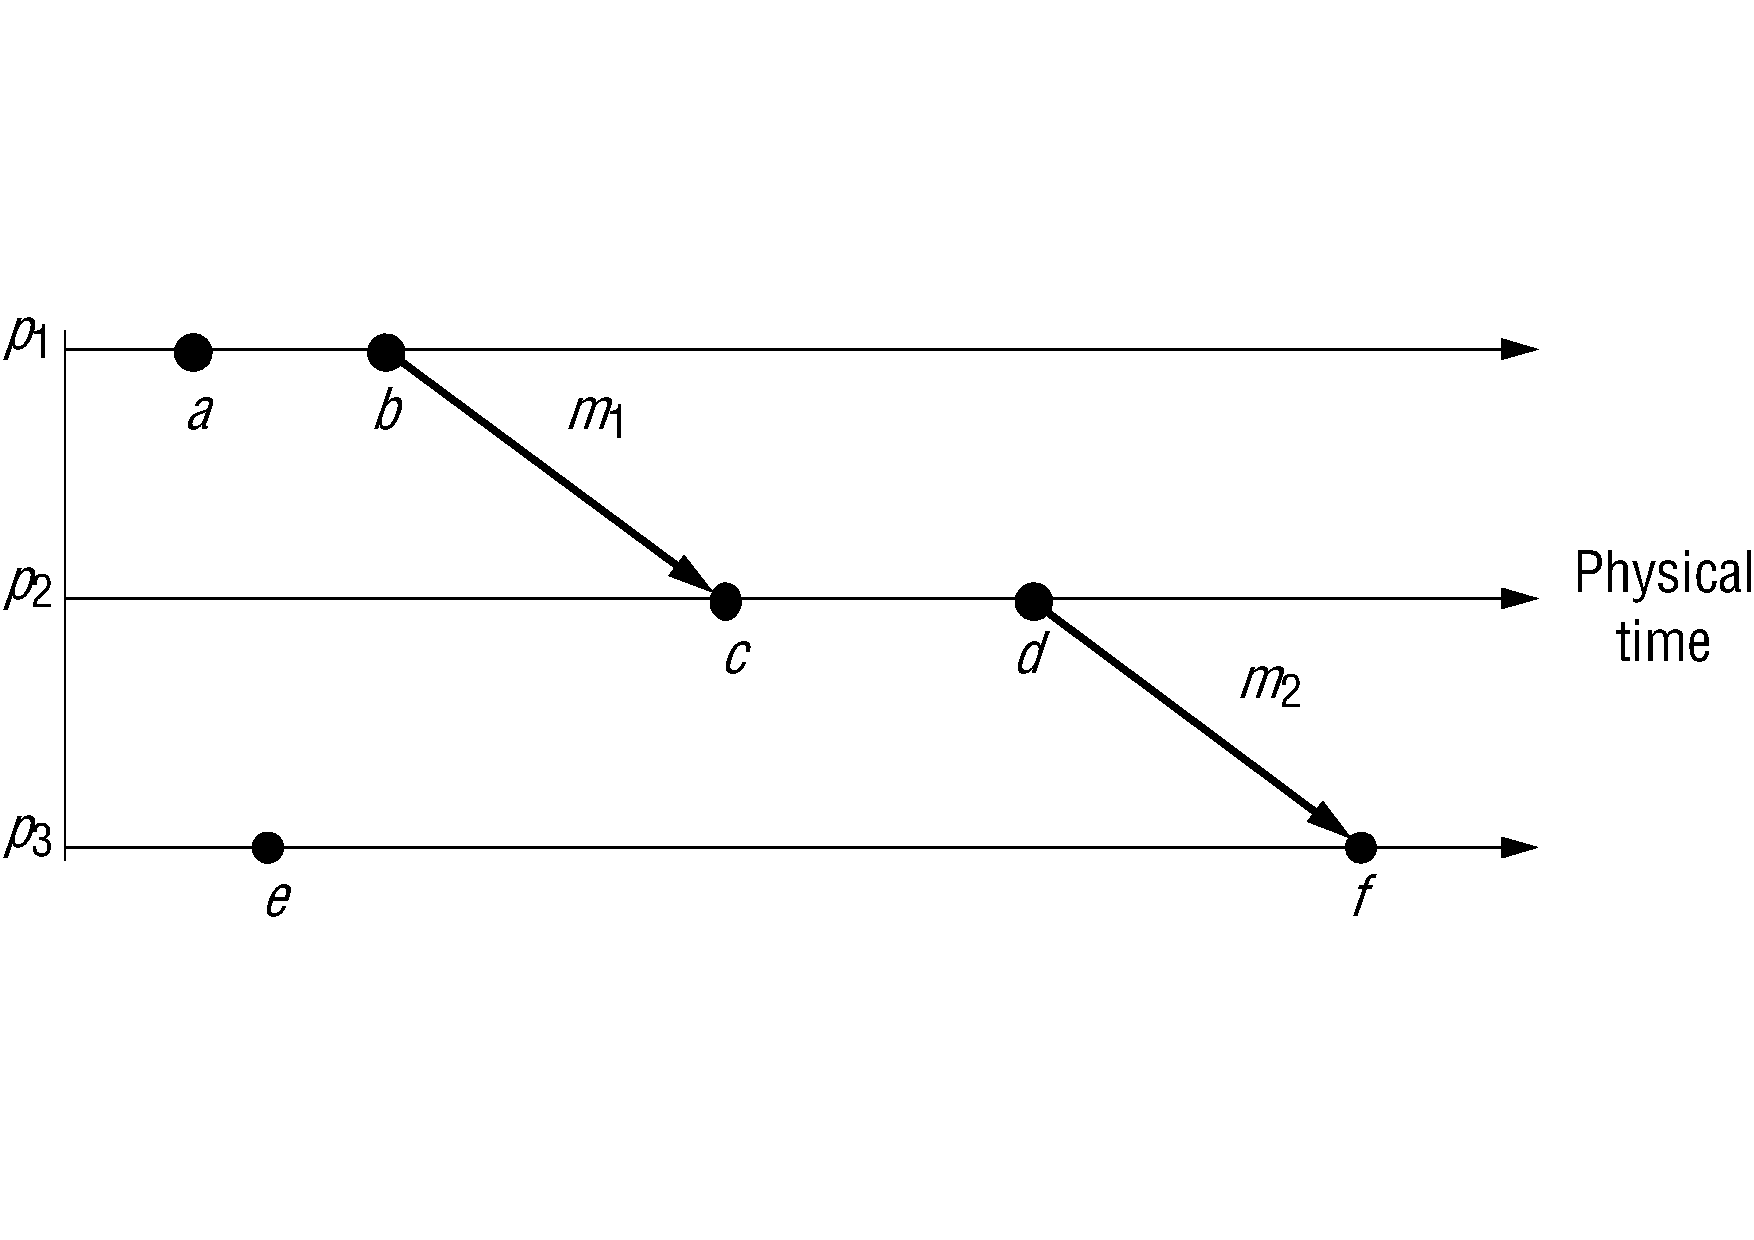
\includegraphics[width=\textwidth]{lamp1}\\
    \vspace{-6em}
  \footnotesize{Fonte: CDKB}
}

\alert{\textbf{Exercício:}} O que se pode dizer sobre:
\begin{enumerate}
\item \textbf{a} e \textbf{b}?
\item \textbf{b} e \textbf{c}?
\item \textbf{a} e \textbf{f}?
\item \textbf{a} e \textbf{e}?
\end{enumerate}

\end{frame}


\section{Relógios Vetoriais}

\begin{frame}
  \frametitle{Relógios vetoriais}
  \begin{block}{Observação:}
    Relógios de Lamport \textbf{não} garantem que $C(a) < C(b)$ implica que $a$ \alert{tenha realmente ocorrido antes} de $b$:
  \end{block}

  \begin{columns}
    \begin{column}{0.4\textwidth}
      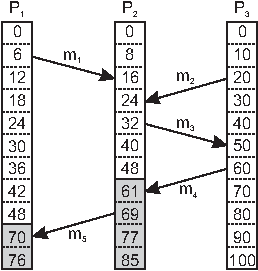
\includegraphics[width=\textwidth]{06-12}
    \end{column}

    \begin{column}{0.5\textwidth}
      \begin{block}{Observação}
        Evento $a$: $m_1$ foi recebido em $T = 16$; \newline
        Evento $b$: $m_2$ foi enviado em $T = 20$.
      \end{block}
    \end{column}
  \end{columns}

  \begin{alertblock}{Nota}
    Nós \alert{não podemos} concluir que $a$ precede temporalmente (precedência causal) $b$.
  \end{alertblock}

\end{frame}

\begin{frame}
  \frametitle{Dependência causal}
  \begin{block}{Definição}
    Dizemos que $b$ pode depender causalmente de $a$ se $ts(a) < ts(b)$ com:
    \begin{itemize}
    \item para todo $k$, $ts(a)[k] \le ts(b)[k]$ e
    \item existe pelo menos um índice $k'$ para o qual $ts(a)[k'] < ts(b)[k']$
    \end{itemize}
  \end{block}

  \begin{block}{Precedência vs.\ dependência}
    \begin{itemize}
    \item Dizemos que $a$ precede causalmente $b$
    \item $b$ \alert{pode} depender causalmente de $a$, já que há informação de $a$ que pode ter sido propagada para $b$
    \end{itemize}
  \end{block}
\end{frame}

\begin{frame}
  \frametitle{Capturando a causalidade - Relógios Vetoriais}
  \alert{Relógios vetoriais foram criados para resolver as limitações
    de relógios de Lamport}, \emph{i.e.}, o fato de que eles
  \textbf{não garantem que se $C(a) < C(b)$ então $a \rightarrow b$}.

\mbox{}

    \begin{block}{Solução: cada $P_i$ mantém um vetor $VC_i$}
      \begin{itemize}
      \item $VC_i[i]$ é o relógio lógico local do processador $P_i$
      \item se $VC_i[j] = k$, então $P_i$ sabe que $k$ eventos ocorreram em $P_j$.
      \end{itemize}
    \end{block}

    \begin{block}{Mantendo os relógios vetoriais}
      \begin{enumerate}
      \item antes da execução de um evento, $P_i$ executa $VC_i[i] \leftarrow VC_i[i]+1$
      \item quando o processo $P_i$ enviar uma mensagem $m$ para $P_j$, ele define o \textit{timestamp} (vetorial) de m $ts(m)$ como sendo $VC_i$ (após executar o passo 1)
      \item no recebimento de uma mensagem $m$, o processo $P_j$ define $VC_j[k] \leftarrow \max\{VC_j[k], ts(m)[k]\}$
      \end{enumerate}
    \end{block}

\end{frame}

\begin{frame}
  \frametitle{Relógios Vetoriais --- Exemplo}

  \begin{onlyenv}<2>
    Suponha agora um atraso no envio de $m_2$:
  \end{onlyenv}

  \begin{figure}
    \centering
    \includegraphics<1->[width=.46\textwidth]{06-13a}
    \qquad
    \includegraphics<2>[width=.46\textwidth]{06-13b}
  \end{figure}

  \begin{block}{Análise}
    \scriptsize
    \begin{tabular}{c|c|c|m{3.5em}|m{3.5em}|l}
      \textbf{Situação} & $ts(m_2)$ & $ts(m_4)$ & $ts(m_2) < ts(m_4)$ & $ts(m_2) > ts(m_4)$ & \textbf{Conclusão} \\ \hline \hline
                        (a)&(2,1,0)&(4,3,0)&Sim&Não&$m_2$ pode preceder causalmente $m_4$, $m_2 \rightarrow m_4$ \\ \hline \pause
                        (b)&(4,1,0)&(2,3,0)&Não&Não&$m_2$ e $m_4$ podem conflitar, $m_2 \parallel m_4$\\ \hline
    \end{tabular}
  \end{block}

\end{frame}

\begin{frame}
  \frametitle{Relógios Vetoriais --- Exercício}
  {\centering
    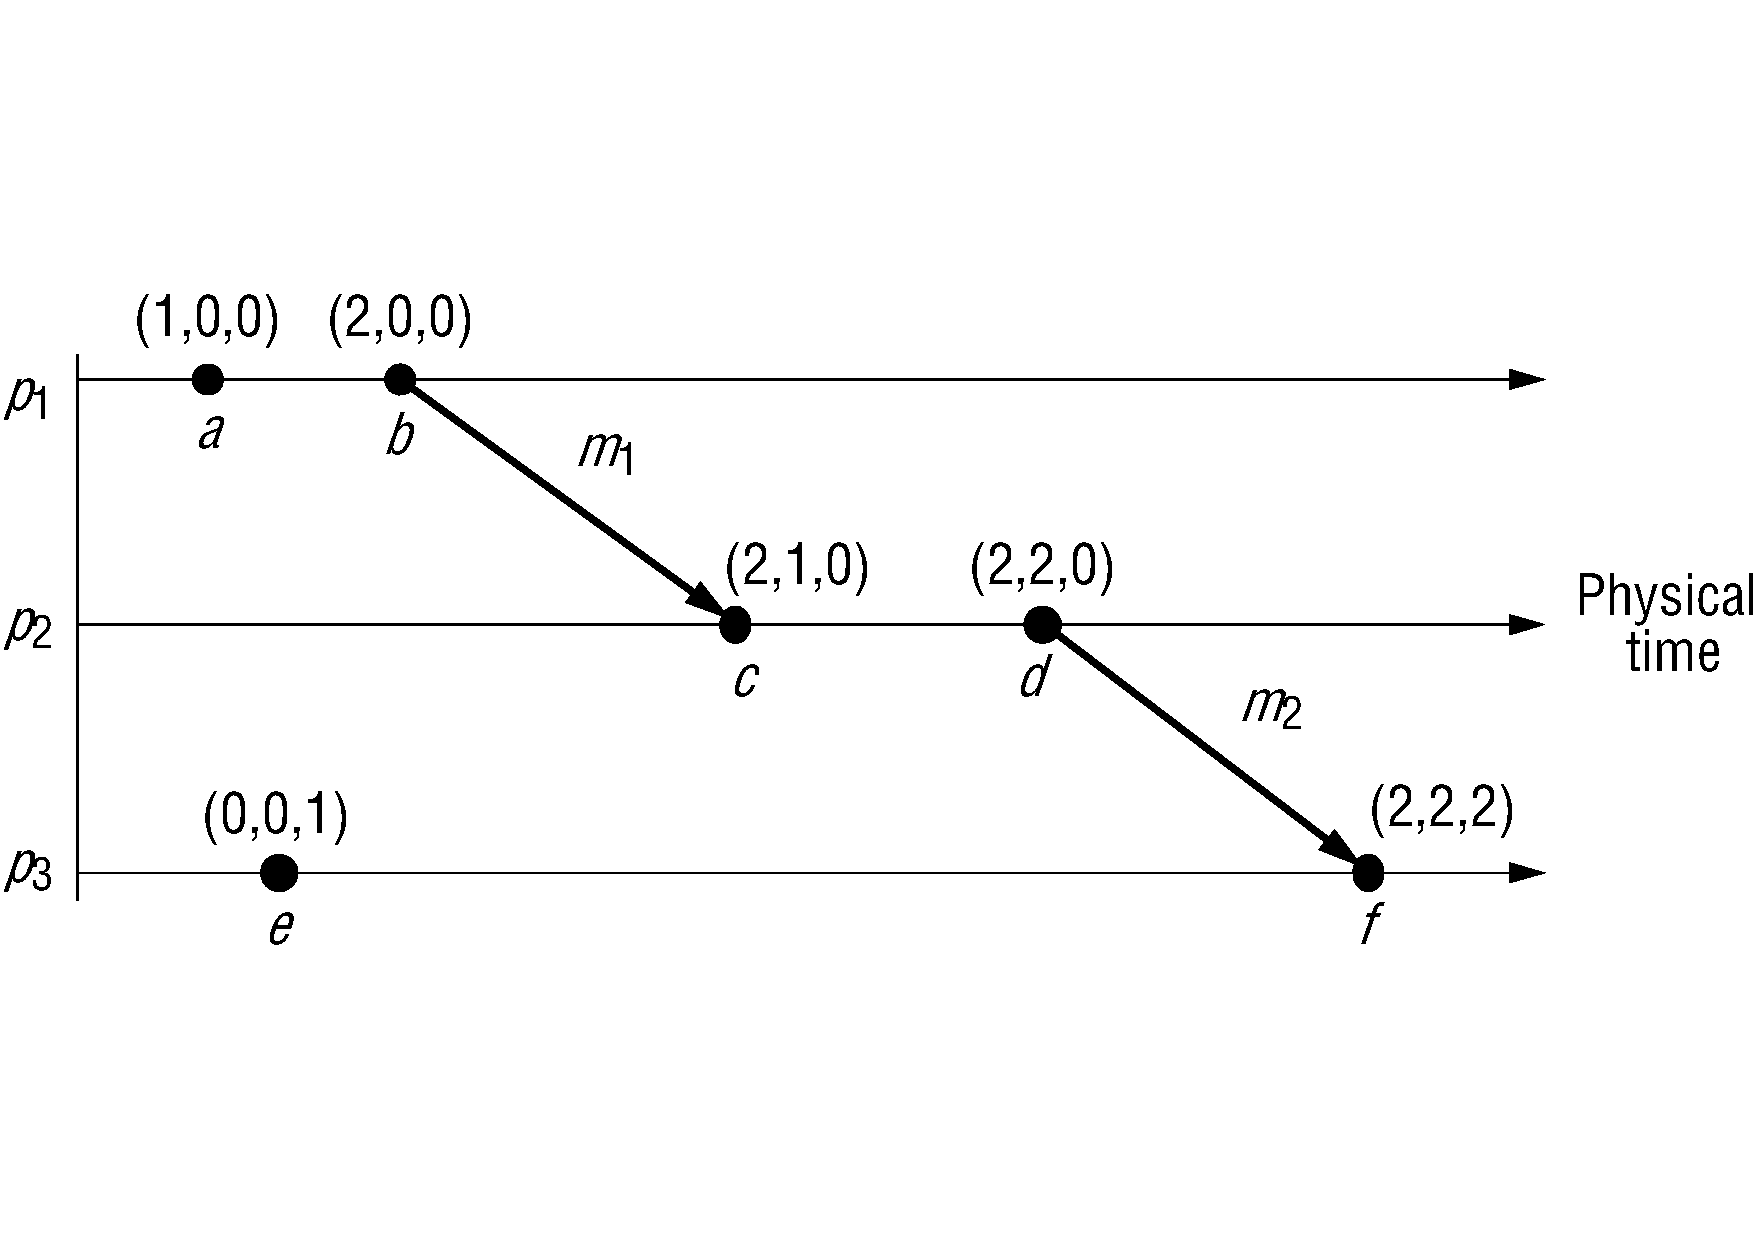
\includegraphics[width=0.9\textwidth]{lamp2}\\
    \vspace{-5em}
    \footnotesize{Fonte: CDKB}
  }

  \alert{\textbf{Exercício}}
  \begin{enumerate}
  \item O que pode ser dito sobre \textbf{a} e \textbf{f}?
  \item O que pode ser dito sobre \textbf{c} e \textbf{e}?
  \end{enumerate}

\end{frame}

\begin{frame}
  \frametitle{Aula passada: multicast com ordem total}
  \begin{alertblock}{Problema}
    Alguma vezes precisamos garantir que atualizações concorrentes em um banco de dados replicado sejam vistos por todos como se tivessem ocorrido na mesma ordem.

  \begin{itemize}
  \item $P_1$ adiciona R\$ 100 a uma conta (valor inicial: R\$ 1000)
  \item $P_2$ incrementa a conta em 1\%
  \item Há duas réplicas
  \end{itemize}
\end{alertblock}

\begin{figure}
  \centering
  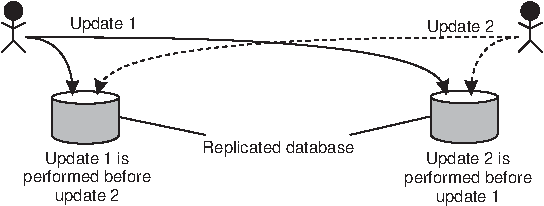
\includegraphics[scale=0.6]{06-11}
\end{figure}

\vspace{-1ex}
\begin{block}{Resultado}
  Na ausência de sincronização correta, \newline réplica \#1 $\leftarrow$ R\$ 1111, enquanto que na réplica \#2 $\leftarrow$ R\$ 1110.
\end{block}

\end{frame}


\begin{frame}
  \frametitle{Multicast ordenado por causalidade}
  \begin{block}{Observação}
    Agora é possível garantir que uma mensagem seja entregue somente
    \textbf{se todas as mensagens que as procederem por causalidade tiverem
    sido entregues}.

    Multicasts \alert{ordenados por causalidade} \textbf{são menos restritivos}
    do que multicasts \emph{com ordem total}. Se
    duas mensagens não tem uma relação causal, então a ordem que elas serão
    entregues pode ser \textbf{diferente para cada um dos processos}.
  \end{block}
\end{frame}

\begin{frame}
  \frametitle{Garantido Multicasts Ordenados por Causalidade}

  Para garantir que as mensagens serão entregues seguindo a ordem causal:

  \begin{block}{Passos}
    \begin{enumerate}
    \item $P_i$ incrementa $VC_i[i]$ somente quando enviar uma mensagem;
    \item $P_j$ \alert{``ajusta''} $VC_j$ quando
      \textbf{entregar}\footnote{\textbf{Atenção}: as mensagens não
        são ajustadas quando são \emph{recebidas}, mas sim quando elas
        são \emph{entregues} à aplicação} uma mensagem (mas não muda
      $VC_j[j]$): $VC_i[k] = \max\{VC_j[k], ts(m)[k]\}, \forall k$
    \end{enumerate}

  \end{block}

  \pause
  \framebox{\begin{minipage}{0.97\textwidth}
      \alert{Além disto, $P_j$ posterga a \textbf{entrega} de $m$ até que}:

      \begin{itemize}
      \item $ts(m)[i] = VC_j[i] + 1$. {\tiny ($m$ é a próxima mensagem que $P_j$ espera de $P_i$)}
      \item $ts(m)[k] \leq VC_j[k]$ para $k \neq i$. {\tiny ($P_j$ já entregou todas as mensagens enviadas para $P_i$)}
      \end{itemize}
    \end{minipage}}

\end{frame}

\begin{frame}
  \frametitle{Multicast ordenado por causalidade}

  \begin{exampleblock}{Exemplo}
    \centering
    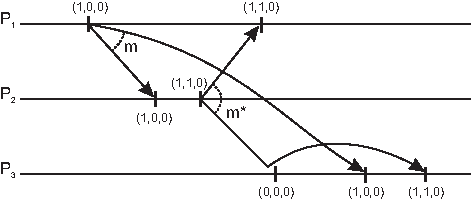
\includegraphics{06-14}
  \end{exampleblock}

  \pause
  \begin{exampleblock}{Exercício}
    Tome $VC_3 = [0,2,2]$, $ts(m) = [1,3,0]$ em $P_1$. Que informação $P_3$ tem e o que ele irá fazer quando receber $m$ (de $P_1$)?
  \end{exampleblock}

\end{frame}

\section{Algoritmos de Exclusão Mútua}

\begin{frame}
  \frametitle{Exclusão mútua}
  \begin{alertblock}{Problema}
    Alguns processos em um sistema distribuído querem acesso exclusivo a algum recurso.
  \end{alertblock}

  \begin{block}{Soluções:}
    \begin{description}
    \item[Baseado em permissão:] um processo que quiser entrar na seção crítica (ou acessar um recurso) precisa da permissão de outros processos
    \item[Baseado em tokens:] um \textit{token} é passado entre processos. Aquele que tiver o \textit{token} pode entrar na seção crítica ou passá-lo para frente quando não estiver interessado.
    \end{description}

    \end{block}

\end{frame}

\begin{frame}
  \frametitle{Baseado em permissão, centralizado}
  \begin{block}{Use um coordenador}
    \begin{figure}
      \centering
      \begin{subfigure}{.3\linewidth}
        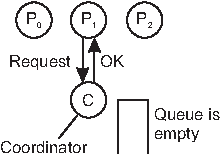
\includegraphics{06-15a}
        \caption{}
      \end{subfigure}
      \quad
      \begin{subfigure}{.3\linewidth}
        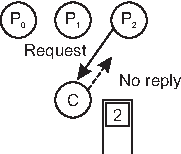
\includegraphics{06-15b}
        \caption{}
    \end{subfigure}
    \quad
      \begin{subfigure}{.3\linewidth}
        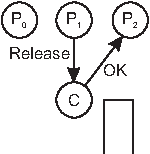
\includegraphics{06-15c}
        \caption{}
      \end{subfigure}
    \end{figure}

    \begin{itemize}
    \item[(a)] Processo $P_1$ pede permissão ao coordenador para acessar o recurso compartilhado. Permissão concedida.
    \item[(b)] Processo $P_2$ então pede permissão para acessar o mesmo recurso. O coordenador não responde.
    \item[(c)] Quando $P_1$ libera o recurso, avisa o coordenador, que então responde para $P_2$.
    \end{itemize}
  \end{block}


\end{frame}

\begin{frame}
  \frametitle{Exclusão mútua -- Ricart \& Agrawala, Versão Distribuída}
  \begin{block}{Princípio}
    Mesmo do Lamport, exceto que acks não são enviados. Ao invés disso, respostas (permissões) são enviadas quando:
    \begin{itemize}
    \item o processo receptor não tem interesse no recurso compartilhado; ou
    \item o processo receptor está esperando por um recurso, mas tem
      menos prioridade (a prioridade é determinada via comparação de
      timestamps)
    \end{itemize}
  \end{block}

    \begin{block}{}
      Em todos os outros casos, o envio da resposta é \alert{adiado}, implicando a necessidade de alguma administração local.
    \end{block}
\end{frame}

\begin{frame}
  \frametitle{Exclusão mútua -- Ricart \& Agrawala, Versão Distribuída}

  Exemplo com três processos:

  \begin{figure}
    \centering
    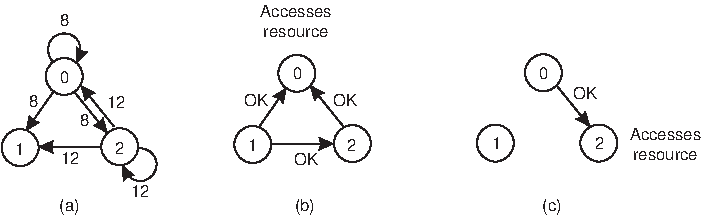
\includegraphics[width=.9\textwidth]{06-15}
  \end{figure}

  \begin{itemize}
  \item[(a)] dois processos ($P_0$ e $P_2$) querem acessar um recurso
    compartilhado ao mesmo tempo
  \item[(b)] $P_0$ tem o menor \textit{timestamp}; ele ganha
  \item[(c)] quando $P_0$ terminar, também manda um OK; assim $P_2$ agora pode continuar
  \end{itemize}

\end{frame}

\begin{frame}
  \frametitle{Exclusão mútua baseada em token}
   \begin{figure}
    \centering
    \begin{minipage}{0.45\textwidth}
      \centering
      
\includegraphics[width=0.9\textwidth]{concha.jpg}\\
      
\includegraphics[width=0.9\textwidth]{concha2.png}
    \end{minipage}\hfill
    \begin{minipage}{0.45\textwidth}
        \centering
        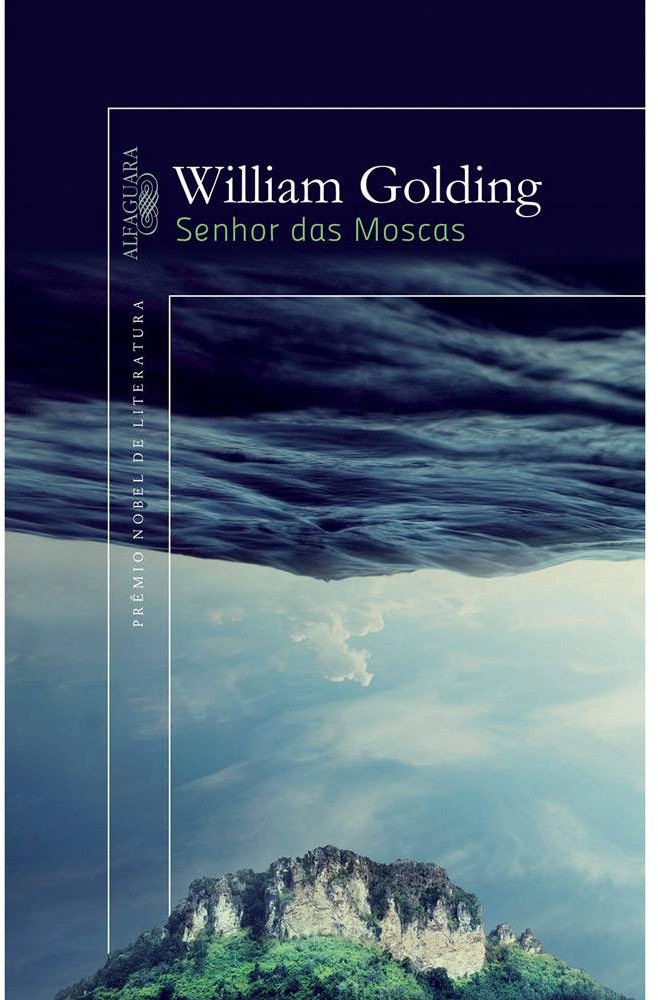
\includegraphics[width=\textwidth]{smoscas.jpg}
    \end{minipage}
  \end{figure}
  \centering
  \footnotesize{Fonte: Google Images}
\end{frame}


\begin{frame}
  \frametitle{Exclusão mútua: token ring}
  \begin{block}{Ideia}
    Organizar os processos em anel \alert{lógico} e passar um \textit{token} entre eles. Aquele que estiver com o \textit{token} pode entrar na seção crítica (se ele quiser).
  \end{block}

  \begin{figure}
    \centering
    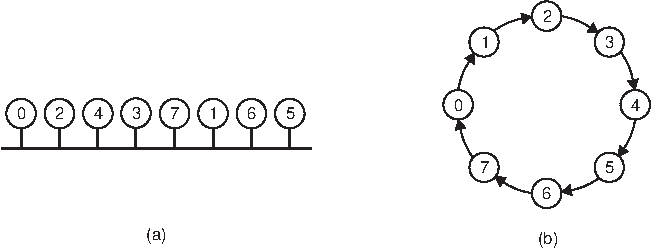
\includegraphics[width=\textwidth]{06-16}
  \end{figure}

\end{frame}

\begin{frame}
  \frametitle{Exclusão mútua decentralizada}
  \begin{block}{Princípio}
    Assuma que todo recurso é replicado $N$ vezes, com cada réplica associada a seu próprio coordenador  $\Rightarrow$ acesso requer a \alert{maioria dos votos} de $m > N/2$ coordenadores. Um coordenador sempre responde imediatamente a uma requisição.
  \end{block}

  \begin{block}{Hipótese}
    Quando um coordenador morrer, ele se recuperará rapidamente, mas terá esquecido tudo sobre as permissões que ele deu.
  \end{block}

\end{frame}

\begin{frame}
  \frametitle{Exclusão mútua decentralizada}

  \begin{block}{Quão robusto é esse sistema?}
    \begin{itemize}
      \item Seja $p = \Delta t / T$ a probabilidade de que um coordenador morra e se recupere em um período $\Delta t$ e que tenha uma esperança de vida $T$.
        \item A probabilidade $\mathbb{P}[k]$ de que $k$ dos $m$ coordenadores sejam resetados durante o mesmo intervalo é:
    \[ \mathbb{P}[k] = \binom{m}{k} p^k (1 - p)^{m-k}\]
  \item $f$ coordenadores resetam $\Rightarrow$ \alert{corretude é violada quando os coordenadores que não falharam são minoria}: quando $m-f \le N/2$ ou $f \ge m-N/2$
  \item A probabilidade de violação é $\sum^N_{m-N/2} \mathbb{P}[k]$.
  \end{itemize}
\end{block}
\end{frame}

\begin{frame}
  \frametitle{Exclusão mútua decentralizada}

    \begin{block}{Probabilidade de violação em função dos parâmetros}
    \begin{center}
      \small\footnotesize
      \renewcommand{\arraystretch}{1.1}
      \begin{tabular}{cc}
        \begin{minipage}{0.4\textwidth}
          \[
          \begin{array}{|c|c|c|c|}\hline
            \mathbf{N}  & \mathbf{m} & \mathbf{p}        & \mbox{\textbf{Violação}} \\ \hline\hline
            8           & 5          & \mbox{3 seg/hora} & < 10^{-15} \\ \hline
            8           & 6          & \mbox{3 seg/hora} & < 10^{-18} \\ \hline
            16          & 9          & \mbox{3 seg/hora} & < 10^{-27} \\ \hline
            16          & 12         & \mbox{3 seg/hora} & < 10^{-36} \\ \hline
            32          & 17         & \mbox{3 seg/hora} & < 10^{-52} \\ \hline
            32          & 24         & \mbox{3 seg/hora} & < 10^{-73} \\ \hline
          \end{array}
          \]
        \end{minipage} &
        \begin{minipage}{0.4\textwidth}
          \[
          \begin{array}{|c|c|c|c|}\hline
            \mathbf{N}  & \mathbf{m} & \mathbf{p}        & \mbox{\textbf{Violação}} \\ \hline\hline
            8           & 5          & \mbox{30 seg/hora} & < 10^{-10} \\ \hline
            8           & 6          & \mbox{30 seg/hora} & < 10^{-11} \\ \hline
            16          & 9          & \mbox{30 seg/hora} & < 10^{-18} \\ \hline
            16          & 12         & \mbox{30 seg/hora} & < 10^{-24} \\ \hline
            32          & 17         & \mbox{30 seg/hora} & < 10^{-35} \\ \hline
            32          & 24         & \mbox{30 seg/hora} & < 10^{-49} \\ \hline
          \end{array}
          \]
        \end{minipage}
      \end{tabular}
    \end{center}
  \end{block}
\end{frame}

\begin{frame}
  \frametitle{Exclusão mútua: comparação}

  \begin{center}
    \footnotesize
    \renewcommand{\arraystretch}{1.2}
    \begin{tabular}{|l|l|l|l|}\hline
      \alert{Algorítimo} 	& \alert{\# msgs por} & \alert{Atraso para entrar} & \alert{Problemas} \\
      & \alert{entrada/saída} & \alert{(em qde msgs)} & \\ \hline
      Centralizado & 3 & 2 & Morte do coordenador \\ \hline
      Decentralizado & 2mk + m, k = 1,2,... & 2mk & \textit{Starvation}, ineficiente.              \\ \hline
      Distribuído & 2~(n~--~1) & 2~(n~--~1) & Morte de qualquer \\ \hline
      Token ring & 1 à $\infty$ & 0 à n~--~1 & Perder token,  proc. morrer\\ \hline
    \end{tabular}
  \end{center}


\end{frame}

\section{Algoritmos de eleição}

\begin{frame}
  \frametitle{Algoritmos de eleição}
  \begin{block}{Princípio}
    Um algoritmo precisa que algum dos processos assuma o papel de coordenador. A pergunta é: como selecionar esse processo especial \alert{dinamicamente}?
  \end{block}

  \begin{block}{Nota}
    Em muitos sistemas o coordenador é escolhido manualmente (ex: servidores de arquivos). Isso leva a soluções centralizadas com um ponto único de falha.
  \end{block}

  \begin{block}{Perguntas}
    \begin{enumerate}
    \item Se um coordenador é escolhido dinamicamente, até que ponto podemos dizer que o sistema será centralizado e não distribuído?
    \item Um sistema inteiramente distribuído (ou seja, um sem um coordenador) é sempre mais robusto que uma solução centralizada/coordenada?
    \end{enumerate}
  \end{block}

\end{frame}

\begin{frame}
  \frametitle{Hipóteses básicas}
  \begin{itemize}
  \item Todos os processos possuem um \texttt{id} único
  \item Todos os processos conhecem os \texttt{id}s de todos os outros processos no sistema (mas eles não tem como saber se os nós estão funcionando ou não)
  \item A eleição significa identificar o processo de maior \texttt{id} que está funcionando em um dado momento
  \end{itemize}
\end{frame}

\begin{frame}
  \frametitle{Algoritmo de eleição --- ``Bully''}

  \begin{block}{Princípio}
    Considere $N$ processos $\{P_0, \ldots, P_{N-1}\}$ e seja $id(P_k)=k$. Quando um processo $P_k$ perceber que o coordenador não está mais respondendo às requisições, ele começa uma nova eleição:
    \begin{enumerate}
    \item $P_k$ envia uma mensagem \texttt{ELECTION} para todos os processos com identificadores maiores que o seu: $P_{k+1}, P_{k+2}, \ldots, P_{N-1}$.
    \item Se ninguém responder, $P_k$ ganha a eleição e se torna o coordenador
    \item Se um dos nós com maior id responder, esse assume\footnote{O maior sempre ganha, por isso o nome de ``algoritmo do valentão''. \fontspec{DejaVu Sans}😜} a eleição e o trabalho de $P_k$ termina.
    \end{enumerate}
  \end{block}

\end{frame}

\begin{frame}
  \frametitle{Algoritmo de eleição --- ``Bully''}

  \begin{figure}
    \centering
    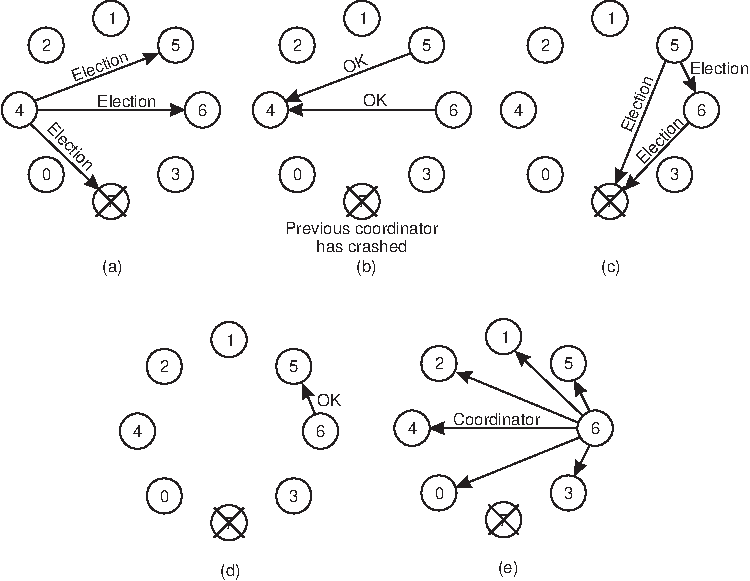
\includegraphics[width=\textwidth]{06-20}
  \end{figure}

\end{frame}

\begin{frame}
  \frametitle{Algoritmo de eleição --- ``Bully''}
  \begin{figure}
    \centering
    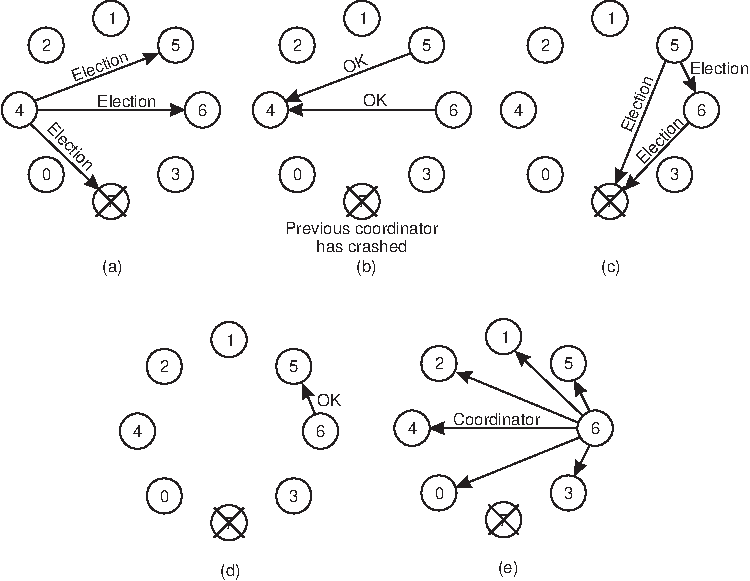
\includegraphics[scale=0.5]{06-20}
  \end{figure}

  \begin{alertblock}{Cuidado}
    Estamos assumido algo importante aqui. O quê? \pause \newline
    Assumimos que a comunicação é \alert{confiável}
  \end{alertblock}

\end{frame}

\begin{frame}
  \frametitle{Eleição em um anel}
  \begin{block}{Princípio}
    As prioridades dos processos são obtidas organizando-os em um anel
    (lógico). Processos com prioridade mais alta devem ser eleitos
    como coordenador.
  \end{block}

  \begin{itemize}
  \item qualquer processo pode iniciar a eleição ao enviar uma
    mensagem de eleição ao seu sucessor. Se um sucessor estiver
    indisponível, a mensagem é enviada ao próximo sucessor
  \item se uma mensagem for repassada, o remetente se adiciona na
    lista. Quando a mensagem voltar ao nó que iniciou, todos tiveram a
    chance de anunciar a sua presença
  \item o nó que iniciou circula uma mensagem pelo anel com a lista de
    nós ``vivos''. O processo com maior prioridade é eleito
    coordenador
  \end{itemize}

\end{frame}

\begin{frame}
  \frametitle{Eleição em um anel}

    \begin{figure}
      \centering
      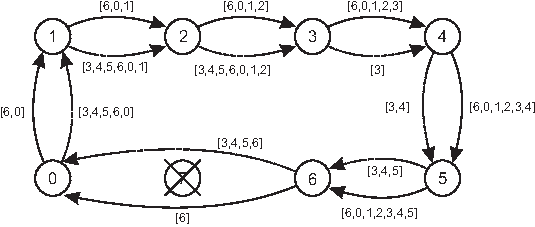
\includegraphics[width=\textwidth]{06-21}
    \end{figure}

    \begin{itemize}
    \item As linhas contíguas mostram as mensagens da eleição iniciada por $P_6$
    \item As linhas pontilhadas se referem a eleição iniciada por $P_3$
    \end{itemize}

\end{frame}

\begin{frame}
  \frametitle{Eleição de um superpeer}
  Como escolher um nó para ser um \alert{superpeer} de forma que:

  \begin{itemize}
  \item nós normais acessem o superpeer com pouca latência
  \item superpeers sejam distribuídos homogeneamente por toda a rede de \textit{overlay}
  \item seja mantida uma fração pré-definida de superpeers em relação ao número total de nós
  \item cada superpeer não deve ter que servir a mais de um número fixo de nós normais
  \end{itemize}
\end{frame}

\begin{frame}
  \frametitle{Eleição de um superpeer}

  \begin{block}{DHTs}
    Reserve uma parte do espaço de IDs para os superpeers. \textbf{Exemplo:} se $S$ superpeers são necessários em um sistema que usa identificadores de $m$-bits, reserve os $k = \lceil \log_2 S \rceil$ bits mais à esquerda para os superpeers. Em um sistema com $N$ nós, teremos, em média, $2^{k-m}N$ superpeers.
  \end{block}

  \begin{block}{Roteamento para superpeers}
    Envie uma mensagem para a chave $p$ para o nó responsável por $p \mbox{\ AND\ } \underbrace{11 \cdots 11}_k \underbrace{00 \cdots 00}_{m-k}$.
  \end{block}
\end{frame}

\section{Sistemas de localização}

\begin{frame}
  \frametitle{Posicionamento dos nós}
  \begin{block}{Problema:}
    Em um sistema distribuído de grande escala onde os nós estão
    dispersados ao longo de uma rede de área ampla (\textit{wide-area
      network}), frequentemente precisamos levar em consideração as
    noções de \alert{proximidade} ou \alert{distância}. Para isso,
    precisamos determinar a \alert{localização} (relativa) de um nó.
  \end{block}

\end{frame}

\begin{frame}
  \frametitle{Cálculo da posição}
  \begin{block}{Observação}
    Um nó $P$ precisa de $d+1$ pontos de referência para calcular sua posição em um espaço $d$-dimensional. Considere o caso bidimensional:
  \end{block}
  \begin{columns}
    \begin{column}{.4\textwidth}
      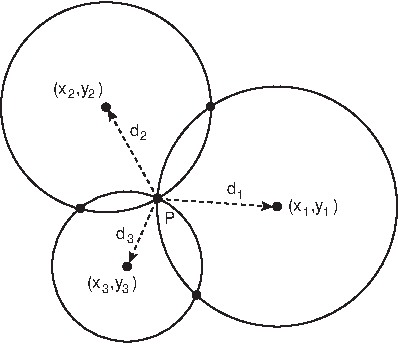
\includegraphics[width=\textwidth]{06-18}
    \end{column}
    \quad
    \begin{column}{.4\textwidth}
      \begin{block}{Solução:}
        $P$ precisa resolver um sistema de três equações com duas incógnitas $(x_P,y_P)$:
        \[ d_i = \sqrt{(x_i-x_P)^2+(y_i-y_P)^2} \]
      \end{block}
    \end{column}
  \end{columns}
\end{frame}

\begin{frame}
  \frametitle{Sistema de posicionamento global}
  \begin{block}{Problema}
    Mesmo assumindo que os relógios dos satélites são precisos e estão sincronizados:
    \begin{itemize}
    \item leva algum tempo até que o sinal chegue ao receptor
    \item o relógio do receptor pode estar totalmente descompassado em relação ao satélite
    \end{itemize}
  \end{block}
\end{frame}

\begin{frame}
  \frametitle{Sistema de posicionamento global}

  \begin{itemize}
  \item \alert{$\Delta_r$}: \alert{defasagem desconhecida} do relógio do receptor
  \item \alert{$x_r$}, \alert{$y_r$}, \alert{$z_r$}: \alert{coordenadas desconhecidas} do receptor
  \item $T_i$: timestamp da mensagem do satélite $i$
  \item $\Delta_i = (T_{agora} - T_i) + \alert{\Delta_r}$: \emph{atraso medido} da mensagem enviada pelo satélite $i$.
  \item \emph{distância \textbf{medida}} do satélite $i$: $c \times \Delta_i$
    \newline ($c$ é a velocidade da luz)
  \item A distância \textbf{real} é:\\
    \[d_i=(T_{agora}- T_i) \times c\]
    logo:
    \[ \alert{d_i} = c \Delta_i - c \alert{\Delta_r} = \sqrt{(x_i - \alert{x_r})^2 + (y_i - \alert{y_r})^2 + (z_i - \alert{z_r})^2}\]

  \end{itemize}

  \begin{block}{Observação}
    4 satélites $\Rightarrow$ 4 equações com 4 incógnitas (\alert{$\Delta_r$} sendo uma delas)
  \end{block}

\end{frame}

\begin{frame}
  \frametitle{Serviços de posicionamento via WiFi}
  \begin{block}{Ideia básica}
    \begin{itemize}
    \item Assuma a existência de um banco de dados com as coordenadas de \textit{access points} (APs) conhecidos
    \item Assuma que podemos estimar a distância até um AP
    \item Então: com três APs detectados, podemos calcular uma posição
    \end{itemize}
  \end{block}
  \begin{block}{Wardriving: localizando os pontos de acesso}
    \begin{itemize}
    \item Use um dispositivo WiFi com um receptor GPS e se mova ao longo de uma área enquanto grava os pontos de acesso
    \item Calcule o centroide: assuma que um ponto de acesso AP foi detectado em $N$ locais diferentes $\{\vec{x_1}, \vec{x_2}, \ldots, \vec{x_N}  \}$ (cujas coordenadas foram capturadas com o GPS)
    \item Calcule a localização do AP como sendo $\vec{X_{AP}} = \frac{\sum_{i=1}^{N} \vec{x_i}}{N}$.
    \end{itemize}
  \end{block}
\end{frame}

\begin{frame}
  \frametitle{Serviços de posicionamento via WiFi}
  \begin{block}{Problemas:}
    \begin{itemize}
    \item acurácia de cada ponto $\vec{x_i}$ detectado pelo GPS
    \item um \textit{access point} tem uma faixa de transmissão que não é uniforme
    \item o número de pontos da amostra ($N$) pode ser muito pequeno
    \end{itemize}
  \end{block}
\end{frame}

% \begin{frame}
%   \frametitle{Exemplos de aplicação}
%   \begin{description}
%   \item[Disseminação de dados] talvez o exemplo mais importante;
%   \item[Agregação] seja $P_i$ um nó que armazena uma variável $v_i$. Quando dois nós se encontrarem, os dois redefinem suas variáveis para
%     \[ v_i,v_j \leftarrow (v_i + v_j)/2 \]
%     Resultado: no final, cada nó terá computado a média aritmética $\overline{v} = \sum_i v_i/N$
%     \begin{itemize}
%     \item O que acontece se os valores forem inicializados com $v_i=1$ e $v_j=0, j \ne i$?
%     \end{itemize}
%   \end{description}
% \end{frame}




\end{document}
